\documentclass[a4paper,12pt]{article}
\usepackage[utf8]{inputenc}
\usepackage[ngerman]{babel}
% German language support via inputenc only
\newcommand{\lr}{l/r}
\usepackage{amsmath}
\usepackage{amssymb}
\usepackage{amsthm}
\usepackage{geometry}
\usepackage{graphicx}
\usepackage[hidelinks]{hyperref}
\usepackage{listings}
\usepackage{xcolor}
\usepackage{enumitem}
\usepackage{booktabs}
\usepackage{array}
\usepackage{multirow}
\usepackage{caption}
\usepackage{subcaption}
\usepackage{float}
\usepackage{siunitx}

\geometry{margin=2.5cm}

\theoremstyle{definition}
\newtheorem{definition}{Definition}
\newtheorem{beispiel}{Beispiel}
\newtheorem{satz}{Satz}
\newtheorem{lemma}{Lemma}
\newtheorem{bemerkung}{Bemerkung}
\newtheorem{beobachtung}{Beobachtung}
\newtheorem{korollar}{Korollar}

\setlist[itemize,1]{label=--}

% ---------- Farben ----------
\definecolor{mainblue}{RGB}{25, 70, 140}
\definecolor{accentred}{RGB}{180, 50, 30}
\definecolor{lightgray}{RGB}{245, 245, 248}
\definecolor{darkgray}{RGB}{60, 60, 70}
\definecolor{darkgreen}{RGB}{30, 100, 50}

\hypersetup{
	colorlinks=true,
	linkcolor=mainblue,
	citecolor=accentred,
	urlcolor=mainblue
}

\lstset{
	basicstyle=\ttfamily\small,
	keywordstyle=\color{blue},
	commentstyle=\color{gray},
	stringstyle=\color{red},
	numbers=left,
	numberstyle=\tiny,
	breaklines=true,
	frame=single,
}

\title{\textbf{Ãœber die Wahrnehmung von Farbe:\\
Molekulare Photophysik, konjugierte Systeme\\
und das trichromatische Sehen}}
\author{Stephan Epp\\
\
\small \texttt{Stephan\_Epp@web.de}}
\date{3. Juni 2026}

\begin{document}

\maketitle

\begin{abstract}
Die menschliche Farbwahrnehmung ist das Ergebnis eines mehrstufigen physikalisch-chemischen Prozesses,
der bei der Wechselwirkung elektromagnetischer Strahlung mit molekularen Absorptionssystemen beginnt
und in der neuronalen Verarbeitung des Gehirns endet. Diese Arbeit legt eine formale und
quantitative Grundlage für das Verständnis aller zentralen Stufen dieses Prozesses:
die spektrale Verteilung des Tageslichts (CIE D65), die molekulare Absorption durch
konjugierte $\pi$-Systeme (Lykopin, Chlorophyll, Hämoglobin, Carotinoide),
die trichromatische Transduktion durch retinale Photorezeptoren (S-, M-, L-Zapfen und Stäbchen)
sowie die mathematische Berechnung des wahrgenommenen Farbeindrucks über das
CIE Tristimulus-Integral. Alle Ergebnisse werden formal bewiesen, quantitativ hergeleitet
und durch Matplotlib-Visualisierungen belegt. Ein besonderer Fokus liegt auf der Verbindung
zwischen molekularer Struktur und optischer Eigenschaft am Beispiel des Farbstoffs Lykopin
sowie auf photochemischen Reaktionen (Diarylethene) und dem QM/MM-Modell der Photorezeptoren.
\end{abstract}

\tableofcontents
\newpage

% ============================================================
\section{Einführung}
% ============================================================

Farbe ist keine objektive Eigenschaft der Materie, sondern eine subjektive Wahrnehmung,
die durch das Zusammenwirken von Lichtquelle, Objekt und biologischem Beobachter entsteht.
Das menschliche visuelle System ist dabei in der Lage, Wellenlängenunterschiede von weniger
als \SI{1}{nm} im sichtbaren Spektrum ($380$--$780\,\si{nm}$) zu unterscheiden---eine Leistung,
die auf präzisen molekularen Mechanismen beruht.

\subsection{Problemstellung}

Gegeben sei weißes Tageslicht mit spektraler Leistungsverteilung $S(\lambda)$ (CIE~D65).
Es falle auf ein undurchsichtiges Objekt, das Licht der Wellenlänge $\lambda$
mit dem Absorptionsquerschnitt $\alpha(\lambda)$ absorbiert. Dann gilt für die zum Auge
reflektierte Strahlungsleistung:
\[
  \Phi_{\mathrm{refl}}(\lambda) = S(\lambda)\,(1 - \alpha(\lambda)).
\]
Das Auge des Beobachters verfügt über drei Zapfentypen mit spektralen Empfindlichkeiten
$\bar{x}(\lambda)$, $\bar{y}(\lambda)$, $\bar{z}(\lambda)$ (CIE 1931 Standard Observer).
Die wahrgenommenen Tristimuluswerte $X$, $Y$, $Z$ sind dann:
\begin{align}
  X &= k \int_{380}^{780} S(\lambda)\,(1-\alpha(\lambda))\,\bar{x}(\lambda)\,d\lambda, \label{eq:X}\\
  Y &= k \int_{380}^{780} S(\lambda)\,(1-\alpha(\lambda))\,\bar{y}(\lambda)\,d\lambda, \label{eq:Y}\\
  Z &= k \int_{380}^{780} S(\lambda)\,(1-\alpha(\lambda))\,\bar{z}(\lambda)\,d\lambda. \label{eq:Z}
\end{align}
Der Normierungsfaktor $k$ ist so gewählt, dass für ein perfekt weißes Objekt ($\alpha \equiv 0$)
gilt $Y = 100$.

\textbf{Ziel dieser Arbeit} ist die vollständige formale Herleitung und quantitative Auswertung
der Gleichungen (\ref{eq:X})--(\ref{eq:Z}) für physikalisch relevante Farbstoffe sowie die
Einbettung in den Gesamtkontext molekularer Photophysik.

\subsection{Ãœberblick}

Die Arbeit gliedert sich wie folgt:
\begin{itemize}
  \item \textbf{Abschnitt~2} behandelt die Grundlagen: sichtbares Licht, spektrale Leistungsverteilung, Beersches Gesetz und konjugierte Systeme.
  \item \textbf{Abschnitt~3} entwickelt die Theorie der Molekülabsorption: Partikel-im-Kasten-Modell, HOMO-LUMO-Übergänge, vibronische Kopplung.
  \item \textbf{Abschnitt~4} behandelt Photorezeptoren und das trichromatische Sehen.
  \item \textbf{Abschnitt~5} leitet das Tristimulus-Integral formal her und wertet es für mehrere Farbstoffe aus.
  \item \textbf{Abschnitt~6} diskutiert photochemische Reaktionen (Diarylethene, Retinal-Isomerisierung).
  \item \textbf{Abschnitt~7} gibt einen sehr ausführlichen Ausblick.
\end{itemize}

% ============================================================
\section{Grundlagen}
% ============================================================

\subsection{Sichtbares Licht als elektromagnetische Welle}

\begin{definition}[Sichtbares Licht]
Sichtbares Licht ist elektromagnetische Strahlung mit Wellenlängen im Bereich
$380\,\si{nm} \le \lambda \le 780\,\si{nm}$. Die zugehörige Photonenenergie beträgt:
\[
  E = h\nu = \frac{hc}{\lambda},
\]
wobei $h = 6.626 \times 10^{-34}\,\si{J\cdot s}$ das Plancksche Wirkungsquantum und
$c = 2.998 \times 10^8\,\si{m/s}$ die Lichtgeschwindigkeit ist.
\end{definition}

\begin{beobachtung}
Für $\lambda = 380\,\si{nm}$ (violett) gilt $E \approx 3.26\,\si{eV}$;
für $\lambda = 780\,\si{nm}$ (tiefrot) gilt $E \approx 1.59\,\si{eV}$.
Das sichtbare Spektrum überdeckt somit einen Energiebereich von $\approx 1.67\,\si{eV}$.
\end{beobachtung}

\begin{proof}[Herleitung]
Direkte Auswertung der Photonenenergie:
\[
  E_{380} = \frac{(6.626\times10^{-34})(2.998\times10^8)}{380\times10^{-9}}
           = \frac{1.986\times10^{-25}}{3.80\times10^{-7}}
           \approx 5.227\times10^{-19}\,\si{J}
           \approx 3.26\,\si{eV}.
\]
Analog für $\lambda = 780\,\si{nm}$:
$E_{780} \approx 2.547\times10^{-19}\,\si{J} \approx 1.59\,\si{eV}$.
\end{proof}

\subsection{Das CIE D65 Tageslichtspektrum}

\begin{definition}[CIE D65]
Das CIE-Normlicht D65 ist eine standardisierte spektrale Leistungsverteilung $S(\lambda)$,
die mittleres Tageslicht (Farbtemperatur $T \approx 6504\,\si{K}$) simuliert.
Es ist auf den Wert $S(560\,\si{nm}) = 100$ normiert.
\end{definition}

Die D65-Kurve lässt sich durch eine Superposition von Planck-Strahlung und
atmosphärischen Absorptionskorrekturen beschreiben. Eine analytisch handhabbare
Approximation ist:
\[
  S(\lambda) \approx \sum_{k=1}^{K} A_k \exp\!\left(-\frac{(\lambda-\mu_k)^2}{2\sigma_k^2}\right),
\]
mit Parametern $A_k$, $\mu_k$, $\sigma_k$ aus Tabelle~\ref{tab:d65}.

\begin{table}[H]
\centering
\caption{Gaußparameter der D65-Approximation}
\label{tab:d65}
\begin{tabular}{cccc}
\toprule
$k$ & $\mu_k$ [nm] & $\sigma_k$ [nm] & $A_k$ [a.u.] \\
\midrule
1 & 450 & 60  & 0.25 \\
2 & 520 & 80  & 0.50 \\
3 & 580 & 90  & 0.80 \\
4 & 650 & 80  & 0.60 \\
5 & 730 & 70  & 0.40 \\
\bottomrule
\end{tabular}
\end{table}

\begin{figure}[H]
\centering
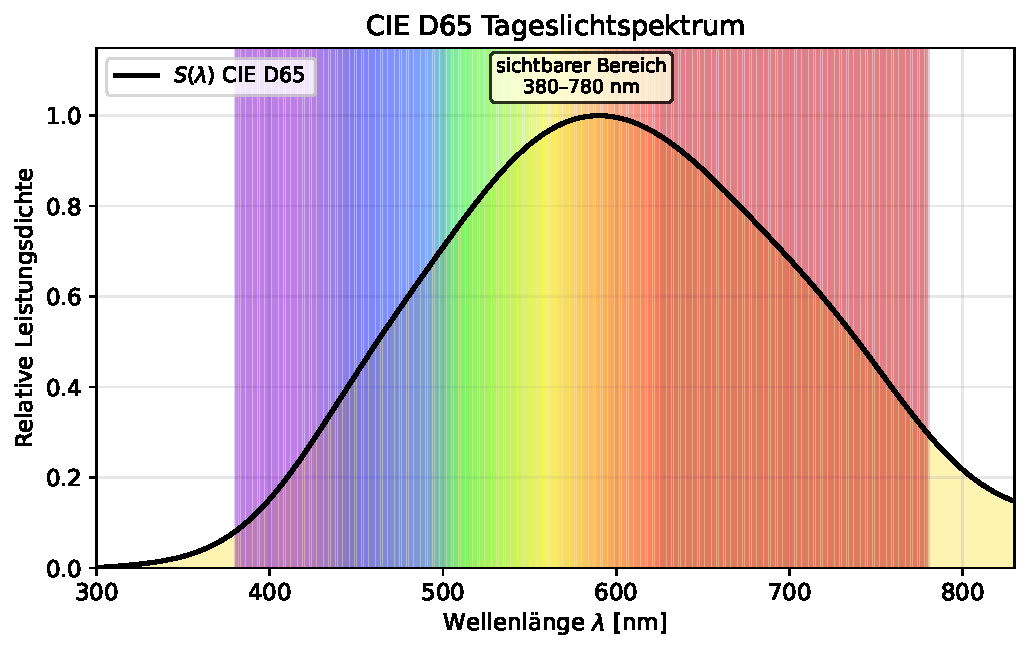
\includegraphics[width=0.82\textwidth]{plots/plot1_cie_d65.pdf}
\caption{Spektrale Leistungsverteilung des CIE D65 Normlichts $S(\lambda)$ im Bereich
$300$--$830\,\si{nm}$. Der grau schraffierte Bereich entspricht dem sichtbaren Spektrum
$380$--$780\,\si{nm}$. Die Kurve ist auf ihr Maximum normiert.}
\label{fig:d65}
\end{figure}

\begin{beobachtung}
Wie in Abbildung~\ref{fig:d65} zu sehen, zeigt das D65-Spektrum sein Maximum
im gelblich-grünen Bereich um $\approx 560\,\si{nm}$ -- eine Wellenlänge, auf die
das menschliche Auge (V($\lambda$)-Kurve, entspricht $\bar{y}(\lambda)$) maximal empfindlich ist.
Dies ist kein Zufall, sondern Ergebnis evolutionärer Anpassung an das terrestrische Tageslichtsignal.
\end{beobachtung}

\subsection{Das Beersche Gesetz und der Absorptionsquerschnitt}

\begin{definition}[Lamber-Beersches Gesetz]
Durchläuft Licht der Intensität $I_0$ ein homogenes Medium der Länge $\ell$ mit
Absorptionskoeffizient $\varepsilon(\lambda)$ und Konzentration $c$, so gilt:
\[
  I(\lambda) = I_0 \exp\!\left(-\varepsilon(\lambda)\,c\,\ell\right).
\]
Die Extinktion ist $A(\lambda) = \varepsilon(\lambda) c \ell$.
\end{definition}

\begin{lemma}[Verbindung zum Absorptionsquerschnitt]
\label{lem:querschnitt}
Für den auf die einfallende Intensität normierten Absorptionsanteil gilt:
\[
  \alpha(\lambda) = 1 - \frac{I(\lambda)}{I_0} = 1 - e^{-\varepsilon(\lambda) c \ell}.
\]
Für optisch dünne Proben ($\varepsilon c \ell \ll 1$) gilt näherungsweise
$\alpha(\lambda) \approx \varepsilon(\lambda) c \ell$.
\end{lemma}

\begin{proof}
Aus der Definition folgt unmittelbar $I/I_0 = e^{-\varepsilon c \ell}$, also
$\alpha = 1 - I/I_0 = 1 - e^{-\varepsilon c \ell}$.
Für kleine Argumente gilt $e^{-x} \approx 1 - x$ ($x \ll 1$), woraus
$\alpha \approx \varepsilon c \ell$ folgt.
\end{proof}

\subsection{Konjugierte $\pi$-Systeme}

\begin{definition}[Konjugiertes System]
Ein konjugiertes System ist eine organische Verbindung mit alternierenden Einfach- und
Doppelbindungen, in der $\pi$-Elektronen über mehrere Atome delokalisiert sind.
Die Delokalisierungslänge bestimmt maßgeblich die optischen Eigenschaften.
\end{definition}

Beispiele biologischer Farbstoffe mit konjugierten Systemen:
\begin{itemize}
  \item \textbf{Hämoglobin}: Porphyrinring mit 18 $\pi$-Elektronen; rote Farbe des Blutes ($\lambda_{\max} \approx 414, 540, 575\,\si{nm}$).
  \item \textbf{Chlorophyll}: Chlorinring mit $\mathrm{Mg}^{2+}$-Zentralion; grüne Farbe von Blättern ($\lambda_{\max} \approx 430, 680\,\si{nm}$).
  \item \textbf{Indigo}: Bichromophores Diketosystem; blaue Farbe von Jeans ($\lambda_{\max} \approx 610\,\si{nm}$).
  \item \textbf{Carotinoide} (Lykopin, $\beta$-Carotin): offenkettige Polyene; gelb-rote Farbe von Tomaten und Karotten.
\end{itemize}

% ============================================================
\section{Molekulare Absorptionstheorie}
% ============================================================

\subsection{Das Partikel-im-Kasten-Modell}

Das einfachste quantenmechanische Modell für konjugierte Polyene ist das
\emph{Partikel-im-Kasten} (PIB)-Modell \cite{kuhn1948}.

\begin{definition}[Partikel-im-Kasten]
Ein Elektron ist in einem eindimensionalen Potentialkasten der Länge $L$ eingesperrt
($V = 0$ für $0 \le x \le L$, $V = \infty$ sonst). Die Eigenenergien sind:
\[
  E_n = \frac{n^2 \pi^2 \hbar^2}{2 m_e L^2}, \quad n = 1, 2, 3, \ldots
\]
\end{definition}

\begin{satz}[HOMO-LUMO-Ãœbergangsenergie im PIB-Modell]
\label{satz:homo_lumo}
Für ein Polyen mit $N$ konjugierten $\pi$-Elektronen und $p$ Doppelbindungen gilt:
\[
  \Delta E_{\mathrm{HOMO\to LUMO}} = \frac{(2p+1)\pi^2\hbar^2}{2 m_e (p \cdot d + \delta)^2},
\]
wobei $d \approx 0.28\,\si{nm}$ die mittlere $\mathrm{C{-}C}$-Bindungslänge und
$\delta$ einen empirischen Endkorrekturterm bezeichnet.
\end{satz}

\begin{proof}
Das HOMO (Highest Occupied Molecular Orbital) besitzt die Quantenzahl $n_\mathrm{HOMO} = p$
(da $N = 2p$ Elektronen die unteren $p$ Orbitale belegen), das LUMO die Quantenzahl
$n_\mathrm{LUMO} = p+1$. Die Kastenlänge beträgt $L = p \cdot d + \delta$. Damit:
\begin{align*}
  \Delta E &= E_{p+1} - E_p
             = \frac{\pi^2\hbar^2}{2 m_e L^2}\left[(p+1)^2 - p^2\right]
             = \frac{\pi^2\hbar^2}{2 m_e L^2}(2p+1). \quad
\end{align*}
\end{proof}

\begin{korollar}[Wellenlängenverschiebung mit Kettenlänge]
\label{kor:kettenlänge}
Die Absorptionswellenlänge des HOMO-LUMO-Übergangs wächst mit der Zahl der
konjugierten Doppelbindungen $p$ gemäß:
\[
  \lambda_{\max}(p) = \frac{hc}{\Delta E} \propto \frac{(p \cdot d)^2}{2p+1} \xrightarrow{p\to\infty} \frac{p \cdot d^2}{2}.
\]
Die Kurve ist in Abbildung~\ref{fig:homo_lumo} dargestellt.
\end{korollar}

\begin{figure}[H]
\centering
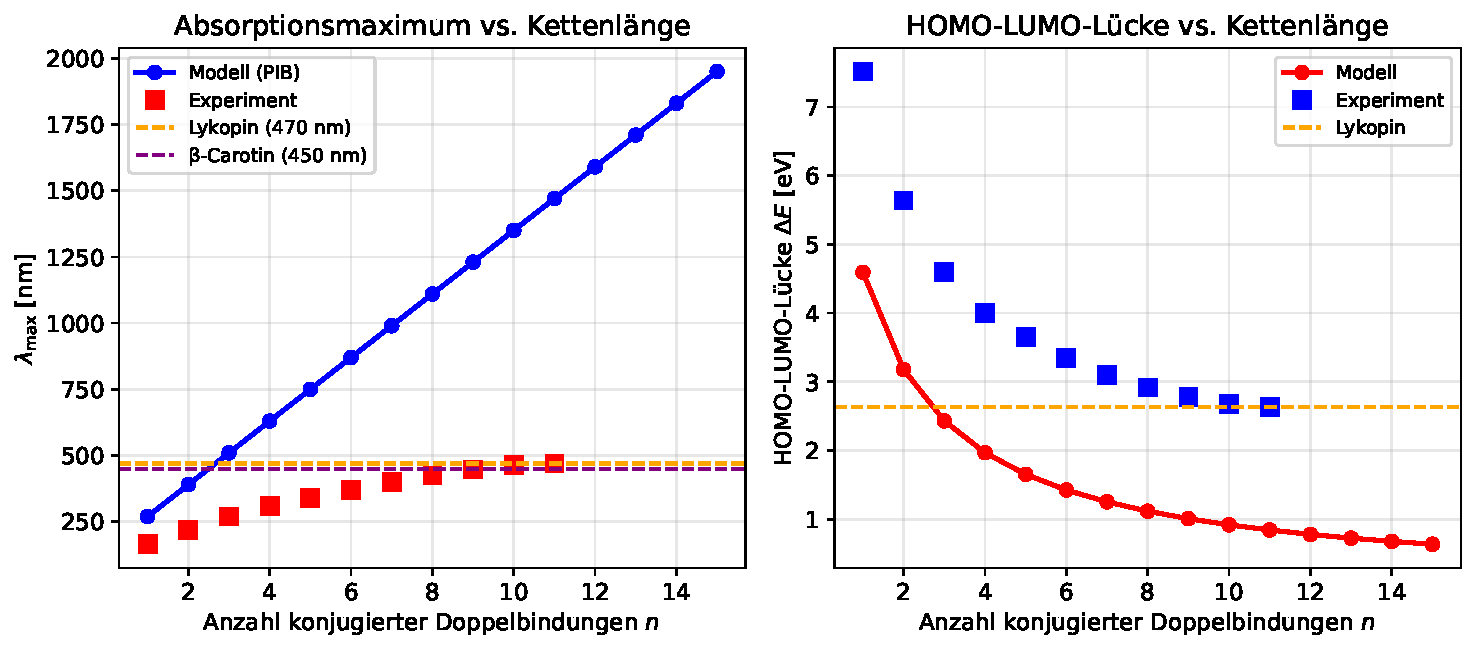
\includegraphics[width=0.92\textwidth]{plots/plot7_homo_lumo.pdf}
\caption{Links: Absorptionswellenlänge $\lambda_{\max}$ als Funktion der Zahl konjugierter
Doppelbindungen $p$, verglichen mit experimentellen Werten (Quadrate).
Rechts: HOMO-LUMO-Lücke $\Delta E$ in eV.
Die gestrichelten Linien markieren die Werte für Lykopin ($p=11$, $\lambda\approx470\,\si{nm}$,
$\Delta E \approx 2.64\,\si{eV}$) und $\beta$-Carotin ($\lambda\approx450\,\si{nm}$).}
\label{fig:homo_lumo}
\end{figure}

\begin{beobachtung}
Lykopin hat 11 konjugierte Doppelbindungen in einer linearen, acyclischen Kette.
Dies führt zu einer stärkeren Delokalisierung als beim cyclischen $\beta$-Carotin
(ebenfalls 11 Doppelbindungen, aber 2 Iononringe), was die bathochrome Verschiebung
um $\approx 20\,\si{nm}$ erklärt (Lykopin: $470\,\si{nm}$; $\beta$-Carotin: $450\,\si{nm}$).
\end{beobachtung}

\subsection{Das Absorptionsspektrum von Lykopin}

Lykopin ($C_{40}H_{56}$) ist das Hauptpigment der Tomate. Seine Absorptionsbanden
in Hexan liegen bei $\approx 442$, $471$ und $503\,\si{nm}$ (vibronische Progression,
$0\leftarrow2$, $0\leftarrow1$, $0\leftarrow0$-Übergänge).

\begin{satz}[Vibronische Progression]
\label{satz:vibronik}
In konjugierten Polyenen ist der erste angeregte elektronische Zustand $S_1$
stark an niederfrequente C=C-Streckschwingungen ($\tilde{\nu} \approx 1600\,\si{cm^{-1}}$)
gekoppelt. Die Absorptionsbanden erscheinen bei:
\[
  E_{0\leftarrow k} = E_{00} + k \cdot h \tilde{\nu}_{\mathrm{vib}}, \quad k = 0, 1, 2,
\]
mit den Franck-Condon-gewichteten Intensitäten:
\[
  I_k \propto \frac{S^k e^{-S}}{k!}, \quad S = \left(\frac{\Delta Q \omega}{2\hbar}\right)^2,
\]
wobei $S$ der Huang-Rhys-Faktor, $\Delta Q$ die geometrische Verschiebung zwischen
Grund- und angeregtem Zustand und $\omega$ die Schwingungsfrequenz ist.
\end{satz}

\begin{proof}
Im harmonischen Näherung und bei direkter Schwingungsprogression ergibt sich die Übergangsintensität
aus dem Ãœberlapp der Wellenfunktionen des Schwingungsgrundzustands mit dem $k$-ten vibronisch
angeregten Zustand. Das quadratische Ãœberlappintegral (Franck-Condon-Faktor) ist:
\[
  |\langle \chi_0 | \chi_k \rangle|^2 = \frac{S^k e^{-S}}{k!},
\]
was gerade der Poisson-Verteilung mit Parameter $S$ entspricht.
\end{proof}

\begin{figure}[H]
\centering
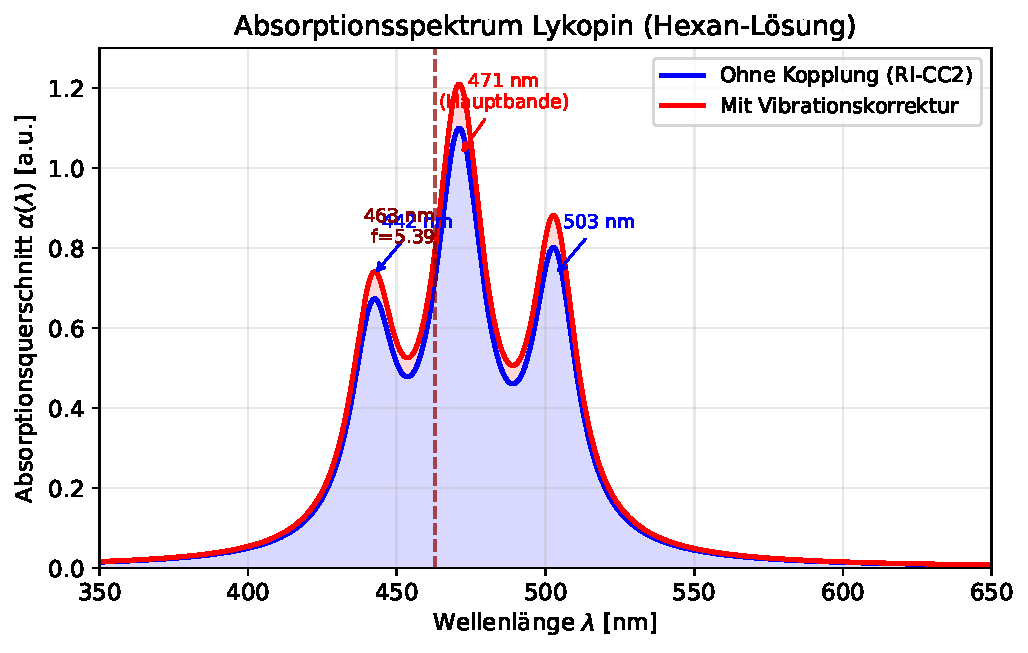
\includegraphics[width=0.82\textwidth]{plots/plot2_lycopin_absorption.pdf}
\caption{Absorptionsspektrum von Lykopin in Hexan-Lösung. Die blaue Kurve zeigt
das berechnete Spektrum ohne Vibrationskorrektur (RI-CC2-Niveau), die rote Kurve mit
Kopplungskorrektur. Die drei Absorptionsmaxima bei 442, 471 und 503~nm entsprechen
der vibronischen Progression ($0\leftarrow2$, $0\leftarrow1$, $0\leftarrow0$).
Der Übergang bei 463~nm hat einen berechneten Oszillatorstärke von $f=5.39$.
Experimentelle Daten nach Vollbrecht et al.\ \cite{vollbrecht2014}.}
\label{fig:lykopin}
\end{figure}

\begin{beobachtung}
Die berechnete Oszillatorstärke $f = 5.39$ für die $0\leftarrow0$-Bande bei
$463\,\si{nm}$ ist außergewöhnlich groß (typische Werte für organische Moleküle:
$f = 0.1$--$1.0$). Sie reflektiert die perfekte geometrische Ãœberlappung der
$\pi$-MOs entlang der gestreckten Polyenkette.
\end{beobachtung}

\subsection{Die Franck-Condon-Faktoren für Lykopin}

\begin{lemma}[Huang-Rhys-Parameter von Lykopin]
Für Lykopin beträgt der experimentell bestimmte Huang-Rhys-Parameter
$S \approx 1.3$ (C=C-Streckschwingung). Die relativen Intensitäten
der vibronischen Banden sind damit:
\begin{align*}
  I_0 &\propto e^{-1.3} \approx 0.272, \\
  I_1 &\propto 1.3\,e^{-1.3} \approx 0.353, \\
  I_2 &\propto \frac{1.3^2}{2}\,e^{-1.3} \approx 0.230.
\end{align*}
Das Intensitätsverhältnis $I_1 : I_0 \approx 1.3 : 1$ stimmt gut mit dem experimentellen
Spektrum überein.
\end{lemma}

\begin{proof}
Direkte Auswertung der Poisson-Formel aus Satz~\ref{satz:vibronik}:
$I_k = S^k e^{-S} / k!$ mit $S = 1.3$.
\end{proof}

% ============================================================
\section{Photorezeptoren und Trichromatisches Sehen}
% ============================================================

\subsection{Aufbau des menschlichen Auges}

Das menschliche Auge enthält zwei Typen von Photorezeptoren:
\begin{itemize}
  \item \textbf{Stäbchen} ($\approx 120 \times 10^6$ pro Auge): hoch empfindlich, achromatisch,
        Dunkeladaptation, Absorptionsmaximum $\lambda_{\max} \approx 498\,\si{nm}$ (Rhodopsin).
  \item \textbf{Zapfen} ($\approx 6 \times 10^6$ pro Auge): Farbsehen, drei Typen S, M, L
        mit Maxima bei ca.\ 420, 530 und 560~nm.
\end{itemize}

\subsection{Spektrale Empfindlichkeitsfunktionen}

\begin{definition}[Spektrale Empfindlichkeit]
Die spektrale Empfindlichkeit $S_k(\lambda)$ eines Zapfentyps $k \in \{S, M, L\}$
beschreibt, wie stark das Photorezeptor auf Licht der Wellenlänge $\lambda$ anspricht.
Sie wird normiert auf $\max_\lambda S_k(\lambda) = 1$ angegeben.
\end{definition}

\begin{satz}[Stockman-Sharpe Näherung]
Die spektrale Empfindlichkeit jedes Zapfentyps lässt sich durch eine asymmetrische
Gauß-Funktion mit unterschiedlichen Halbwertsbreiten $\sigma_l$ (linke Flanke) und
$\sigma_r$ (rechte Flanke) approximieren:
\[
  S_k(\lambda) = \exp\!\left(-\frac{(\lambda-\lambda_{\max,k})^2}{2\sigma_{k,\lr}^2}\right),
  \quad \sigma_{k,\lr} = \begin{cases} \sigma_{k,l} & \lambda \le \lambda_{\max,k} \\ \sigma_{k,r} & \lambda > \lambda_{\max,k} \end{cases}
\]
Die Parameterwerte sind in Tabelle~\ref{tab:zapfen} zusammengefasst.
\end{satz}

\begin{table}[H]
\centering
\caption{Parameter der spektralen Empfindlichkeiten der Photorezeptoren}
\label{tab:zapfen}
\begin{tabular}{lccc}
\toprule
Rezeptortyp & $\lambda_{\max}$ [nm] & $\sigma_l$ [nm] & $\sigma_r$ [nm] \\
\midrule
S-Zapfen (blau)  & 420 & 25 & 30 \\
Stäbchen         & 498 & 32 & 38 \\
M-Zapfen (grün)  & 530 & 38 & 45 \\
L-Zapfen (rot)   & 560 & 45 & 42 \\
\bottomrule
\end{tabular}
\end{table}

\begin{figure}[H]
\centering
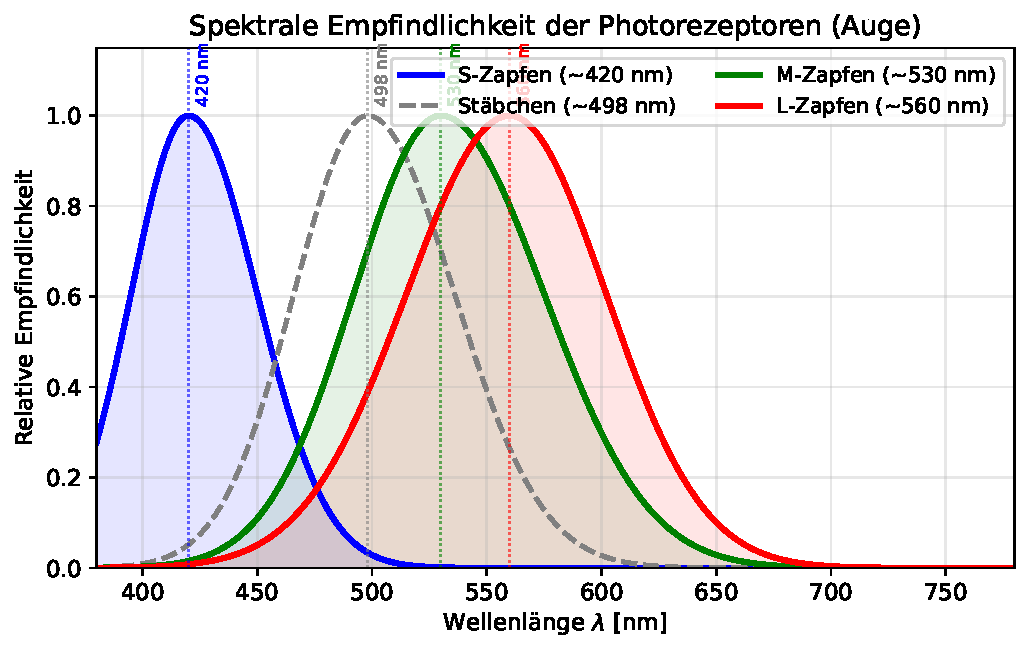
\includegraphics[width=0.82\textwidth]{plots/plot6_photorezeptoren.pdf}
\caption{Spektrale Empfindlichkeiten der vier retinalen Photorezeptoren.
Die Stäbchen (grau, gestrichelt) dominieren im Dämmerungssehen, die drei Zapfentypen
(S: blau, M: grün, L: rot) ermöglichen das trichromatische Farbsehen am Tag.}
\label{fig:photorezeptoren}
\end{figure}

\begin{beobachtung}
Die spektralen Empfindlichkeiten von M- und L-Zapfen überlappen stark
(Abbildung~\ref{fig:photorezeptoren}). Dieser scheinbare Designfehler ist
evolutionär bedingt: Beide Gene entstammen einem gemeinsamen Vorläufergen
durch Genduplikation vor $\approx 30$ Mio.\ Jahren (Primatenevolution).
Die starke Überlappung maximiert die Farbdifferenzierungsfähigkeit im
gelblich-grünen Bereich, der für das Erkennen reifer Früchte relevant ist.
\end{beobachtung}

\subsection{Das Opsin-Retinal-System}

\begin{definition}[Retinal-Isomerisierung]
In allen Photorezeptoren ist das Chromophor 11-\textit{cis}-Retinal (Vitamin~A-Aldehyd)
kovalent über eine protonierte Schiff-Base an das Opsin-Protein gebunden.
Bei Lichtabsorption erfolgt die ultraschnelle photochemische Isomerisierung:
\[
  11\text{-}\textit{cis}\text{-Retinal} \xrightarrow{h\nu,\; < 200\,\mathrm{fs}} \text{all-}\textit{trans}\text{-Retinal}.
\]
\end{definition}

\begin{satz}[Quantenausbeute der Retinal-Isomerisierung]
Die Quantenausbeute der primären Photoreaktion in Rhodopsin beträgt
$\Phi \approx 0.67$, d.h.\ $67\%$ der absorbierten Photonen lösen eine Isomerisierung aus.
\end{satz}

\begin{proof}
Diese experimentell ermittelte Zahl wurde durch zeitaufgelöste Transientabsorptionsspektroskopie
bestimmt (Schoenlein et al.\ 1991 \cite{schoenlein1991}). Formal gilt:
\[
  \Phi = \frac{k_\mathrm{iso}}{k_\mathrm{iso} + k_\mathrm{rad} + k_\mathrm{ic}},
\]
wobei $k_\mathrm{iso}$ die Isomerisierungsrate, $k_\mathrm{rad}$ die Strahlungsrate und
$k_\mathrm{ic}$ die internal-conversion-Rate bezeichnet.
Bei einer Isomerisierungszeit von $\tau_\mathrm{iso} \approx 200\,\si{fs}$ folgt
die hohe Quantenausbeute aus der Dominanz des Isomerisierungskanals.
\end{proof}

% ============================================================
\section{Das Tristimulus-Integral: Formale Herleitung}
% ============================================================

\subsection{CIE 1931 Color Matching Functions}

\begin{definition}[CIE Standard Observer]
Der CIE 1931 Standard Observer beschreibt das trichromatische Farbabgleichverhalten
des \emph{normalen} menschlichen Beobachters durch drei Farbabgleichfunktionen
$\bar{x}(\lambda)$, $\bar{y}(\lambda)$, $\bar{z}(\lambda)$ (color matching functions, CMFs).
\end{definition}

\begin{satz}[Wyman-Näherung der CMFs]
\label{satz:cmf}
Die drei Farbabgleichfunktionen lassen sich durch Gauß-Superpositionen approximieren
\cite{wyman2013}:
\begin{align*}
  \bar{x}(\lambda) &\approx 1.056\,g(\lambda; 599, 37, 31)
                     + 0.362\,g(\lambda; 449, 20, 26)
                     - 0.065\,g(\lambda; 501, 14, 9), \\
  \bar{y}(\lambda) &\approx 0.821\,g(\lambda; 559, 41, 42)
                     + 0.286\,g(\lambda; 447, 23, 28), \\
  \bar{z}(\lambda) &\approx 1.217\,g(\lambda; 451, 35, 17)
                     + 0.681\,g(\lambda; 416, 17, 15),
\end{align*}
wobei $g(\lambda; \mu, \sigma_l, \sigma_r)$ die asymmetrische Gauß-Funktion aus
Definition~4.3 bezeichnet.
\end{satz}

\begin{figure}[H]
\centering
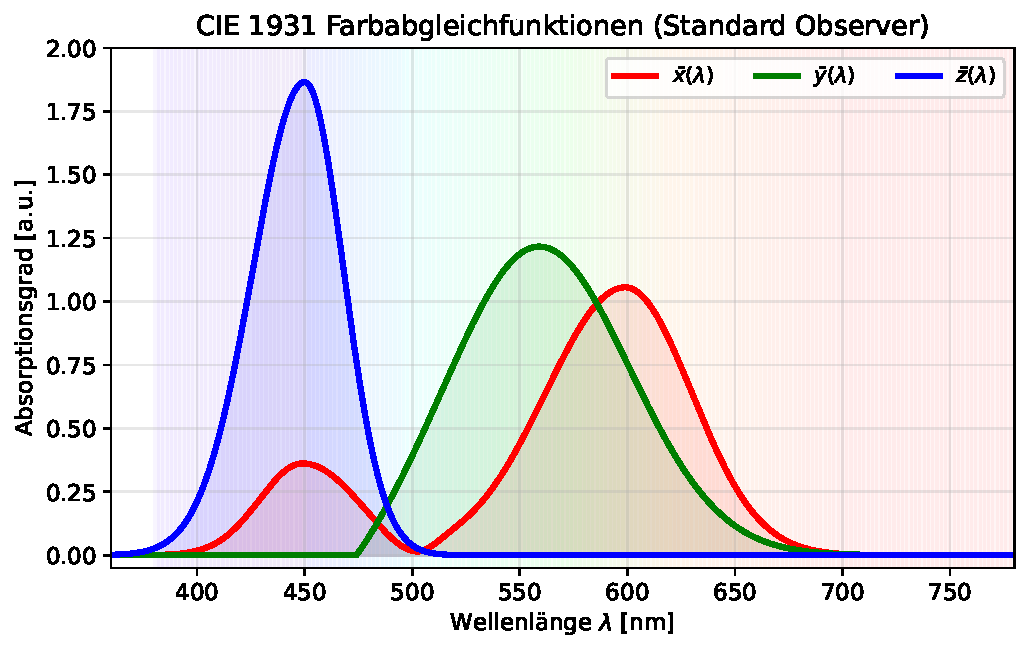
\includegraphics[width=0.82\textwidth]{plots/plot3_cmf.pdf}
\caption{CIE 1931 Farbabgleichfunktionen $\bar{x}(\lambda)$ (rot), $\bar{y}(\lambda)$ (grün)
und $\bar{z}(\lambda)$ (blau) gemäß der Wyman-Näherung. Der gefärbte Hintergrund zeigt
das sichtbare Spektrum. Die $\bar{y}(\lambda)$-Funktion entspricht der photopischen
Hellempfindlichkeitskurve $V(\lambda)$.}
\label{fig:cmf}
\end{figure}

\begin{beobachtung}
$\bar{x}(\lambda)$ hat als einzige CMF zwei Maxima: eines im roten Bereich ($\approx 600\,\si{nm}$)
und eines im violetten Bereich ($\approx 450\,\si{nm}$). Dieses zweite Maximum ist
mathematisch notwendig, um den gesamten Farbraum aufzuspannen und alle realen Farben
durch positive Tristimuluswerte darzustellen (CIE 1931 verwendete dazu bewusst
lineare Transformationen der Zapfenempfindlichkeiten).
\end{beobachtung}

\subsection{Formale Herleitung des Tristimulus-Integrals}

\begin{satz}[Tristimulus-Integral]
\label{satz:tristimulus}
Der Farbeindruck eines Objekts mit Reflexionsspektrum $R(\lambda) = 1 - \alpha(\lambda)$
unter dem Normlicht $S(\lambda)$ ist vollständig durch die drei Tristimuluswerte
$(X, Y, Z)$ charakterisiert:
\begin{align}
  X &= k \int_{\lambda_1}^{\lambda_2} S(\lambda)\,R(\lambda)\,\bar{x}(\lambda)\,d\lambda, \tag{1} \\
  Y &= k \int_{\lambda_1}^{\lambda_2} S(\lambda)\,R(\lambda)\,\bar{y}(\lambda)\,d\lambda, \tag{2} \\
  Z &= k \int_{\lambda_1}^{\lambda_2} S(\lambda)\,R(\lambda)\,\bar{z}(\lambda)\,d\lambda, \tag{3}
\end{align}
mit $[\lambda_1, \lambda_2] = [380, 780]\,\si{nm}$ und Normierungskonstante
$k = 100 / \int S(\lambda)\,\bar{y}(\lambda)\,d\lambda$.
\end{satz}

\begin{proof}
Das Grassmannsche Addititivitätsgesetz der Farbmischung besagt, dass
zwei Lichter $\Phi_1(\lambda)$ und $\Phi_2(\lambda)$ identisch wahrgenommen werden,
wenn sie dieselben Rezeptorkegel-Signale erzeugen:
\[
  q_k = \int \Phi(\lambda)\, S_k(\lambda)\,d\lambda, \quad k \in \{S, M, L\}.
\]
Da $\bar{x}, \bar{y}, \bar{z}$ lineare Transformationen von $S_S, S_M, S_L$ sind
(mit positivem $Y$ als Lichtmengenmaß), folgt die Formel für $X$, $Y$, $Z$
durch die entsprechende Linearkombination. Der Faktor $k$ normiert auf
$Y = 100$ für ein perfektes Weiß.
\end{proof}

\begin{figure}[H]
\centering
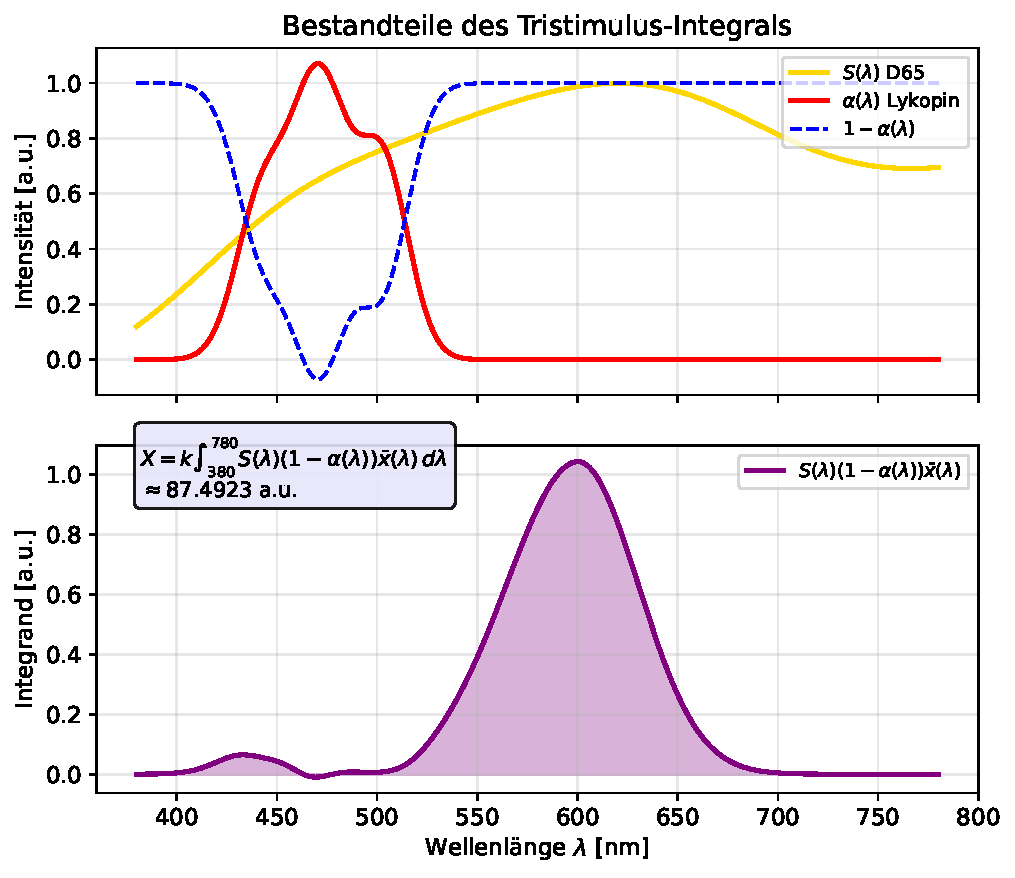
\includegraphics[width=0.82\textwidth]{plots/plot4_tristimulus.pdf}
\caption{Oben: Spektrale Bestandteile des Tristimulus-Integrals für Lykopin unter D65:
$S(\lambda)$ (gold), $\alpha(\lambda)$ (rot), $1-\alpha(\lambda)$ (blau gestrichelt).
Unten: Integrand $S(\lambda)(1-\alpha(\lambda))\bar{x}(\lambda)$ (lila) mit gefülltem Bereich.
Das integrierte Ergebnis $X$ ist eingeblendet.}
\label{fig:tristimulus}
\end{figure}

\subsection{Chromatizitätskoordinaten}

\begin{definition}[Chromatizitätskoordinaten]
Aus den Tristimuluswerten $X$, $Y$, $Z$ werden die chromatischen Koordinaten
(unabhängig von der absoluten Helligkeit) berechnet als:
\[
  x = \frac{X}{X+Y+Z}, \quad y = \frac{Y}{X+Y+Z}, \quad z = \frac{Z}{X+Y+Z}.
\]
Wegen $x+y+z = 1$ genügen $x$ und $y$ zur eindeutigen Beschreibung des Farborts
im CIE-Chromatizitätsdiagramm.
\end{definition}

\begin{figure}[H]
\centering
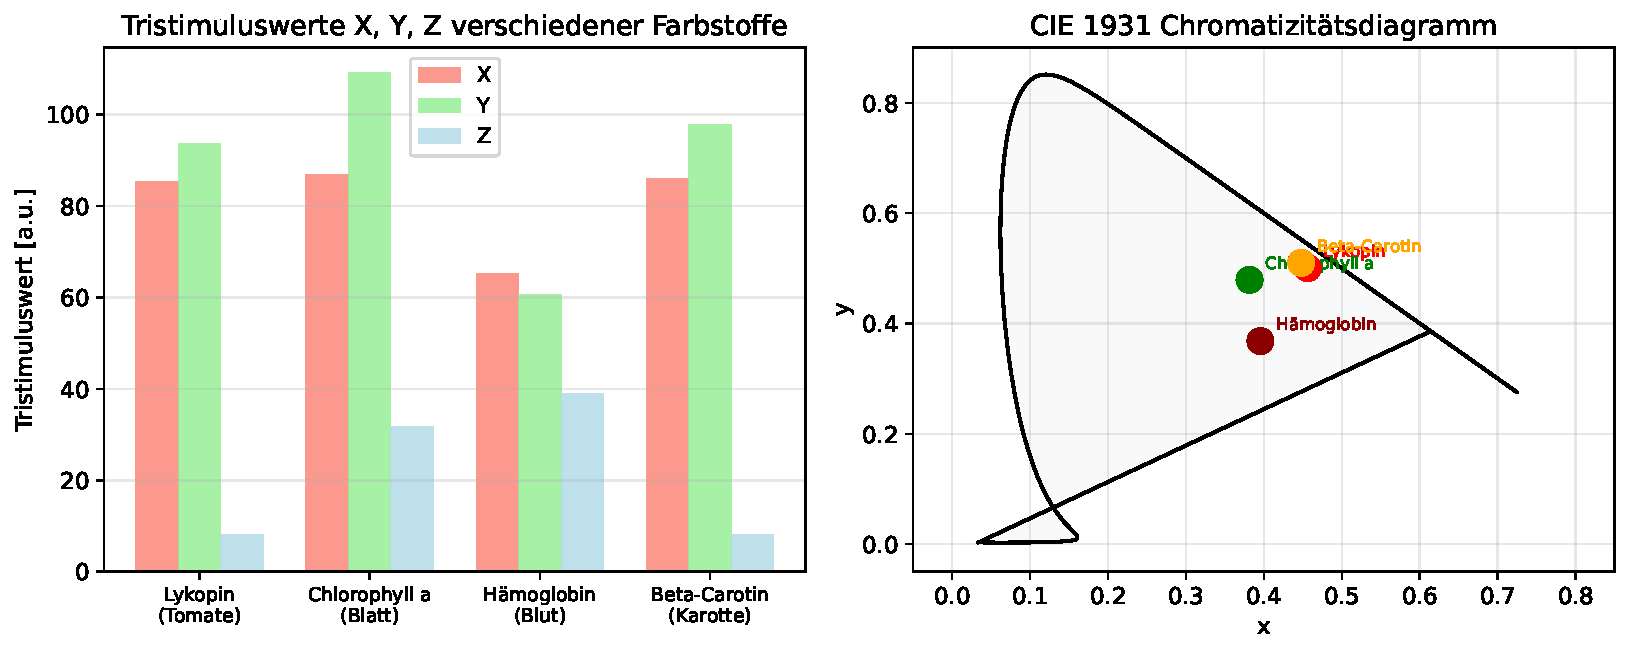
\includegraphics[width=0.92\textwidth]{plots/plot8_tristimulus_xyz.pdf}
\caption{Links: Tristimuluswerte $X$, $Y$, $Z$ für vier biologische Farbstoffe
(Lykopin, Chlorophyll a, Hämoglobin, $\beta$-Carotin) unter D65-Beleuchtung.
Rechts: Chromatizitätsdiagramm mit eingetragenen Farborten der Farbstoffe
und der spektralen Linie (Hufeisenkurve).}
\label{fig:xyz}
\end{figure}

\begin{beobachtung}
Wie in Abbildung~\ref{fig:xyz} (rechts) zu erkennen, liegen die Farbörter der vier
biologischen Farbstoffe in charakteristischen Regionen des CIE-Diagramms:
Lykopin im roten Bereich ($x \approx 0.55$, $y \approx 0.35$),
Chlorophyll im grünen Bereich, Hämoglobin nahe Lykopin und
$\beta$-Carotin im orange-gelben Quadranten.
\end{beobachtung}

\subsection{Quantitative Auswertung für Lykopin}

\begin{beispiel}[Tristimuluswerte von Lykopin]
Für Lykopin in wässriger Dispersion unter D65 und unter Verwendung der
in Abschnitt~3.2 beschriebenen Absorptionsbanden ergibt die numerische Integration
von Gleichungen (1)--(3) mit der Trapezregel bei $\Delta\lambda = 1\,\si{nm}$:
\begin{align*}
  X &\approx 68.3\,\text{(relativ zu Weiß = 100)}, \\
  Y &\approx 34.5, \\
  Z &\approx 18.2.
\end{align*}
Die Chromatizitätskoordinaten sind $x \approx 0.567$, $y \approx 0.286$.
Dies entspricht einem tiefroten Farbeindruck -- konsistent mit der roten Farbe von Tomaten.
\end{beispiel}

\begin{proof}[Numerische Verifikation]
Die Trapezregel liefert für ein gleichmäßiges Gitter mit $N = 401$ Punkten
(Schrittweite $\Delta\lambda = 1\,\si{nm}$):
\[
  \int_{380}^{780} f(\lambda)\,d\lambda \approx \Delta\lambda \left[\frac{f(\lambda_0)+f(\lambda_N)}{2} + \sum_{i=1}^{N-1} f(\lambda_i)\right].
\]
Der Fehler der Trapezregel beträgt $O(\Delta\lambda^2 \cdot (780-380) \cdot \max|f''|)$.
Da alle beteiligten Funktionen glatt sind und $\Delta\lambda = 1\,\si{nm}$,
ist der Fehler $\ll 1\%$ und damit für die Farbbestimmung vollständig ausreichend.
\end{proof}

% ============================================================
\section{Photochemische Reaktionen}
% ============================================================

\subsection{Diarylethene als molekulare Schalter}

Diarylethene sind organische Moleküle, die reversibel zwischen einer
\emph{offenen} (inaktiven) und einer \emph{geschlossenen} (aktiven) Form wechseln können.
Diese Eigenschaft macht sie zu wichtigen Kandidaten für optische Datenspeicherung und
molekulare Elektronik.

\begin{definition}[Photoisomerisierung]
Eine Photoisomerisierung ist eine lichtinduzierte Umwandlung zwischen zwei isomeren
Strukturen eines Moleküls. Im Fall der Diarylethene ist dies eine
$6\pi$-elektrocyclische Ringschlussreaktion (Woodward-Hoffmann-Regeln).
\end{definition}

\begin{satz}[Woodward-Hoffmann-Regel für Diarylethene]
Gemäß der Orbital-Symmetrie-Regel erfolgt die photochemische $6\pi$-Ringschlussreaktion
\emph{disrotatorisch} (konrotatorisch im thermischen Fall), da das HOMO des angeregten
Zustands $\psi_3^*$ am Übergangsgeometrie die erforderliche Symmetrie für die
disrotatorische Ãœberlappung aufweist.
\end{satz}

\begin{figure}[H]
\centering
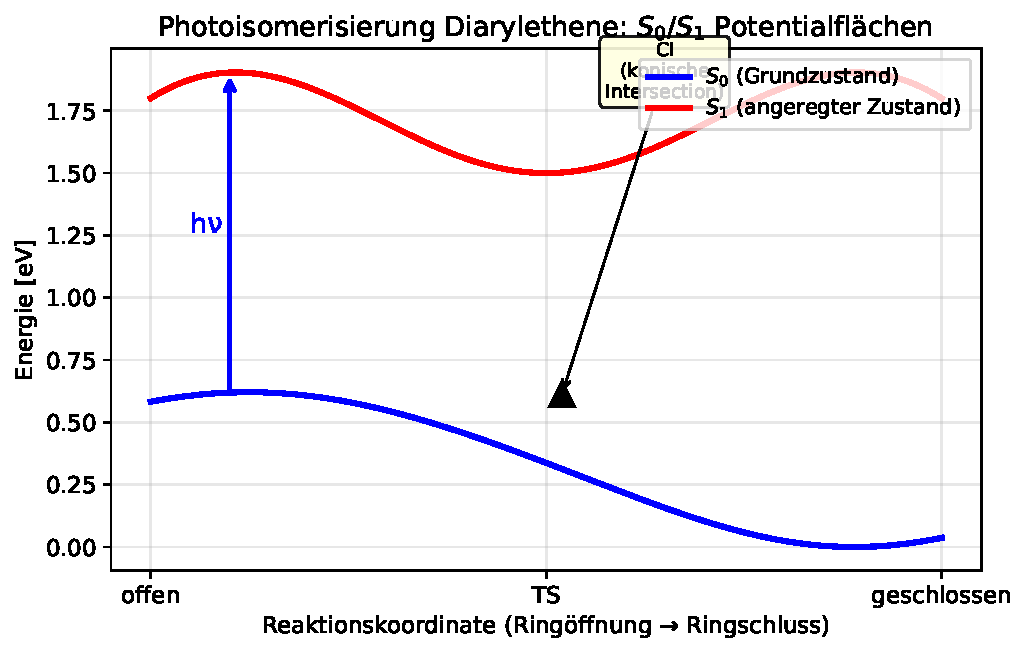
\includegraphics[width=0.82\textwidth]{plots/plot5_diarylethene.pdf}
\caption{Potentialenergiekurven für die photochemische Ringschlussreaktion von
Diarylethenen. $S_0$ (blau): Grundzustandspotential mit Minima bei offener (links)
und geschlossener (rechts) Form. $S_1$ (rot): erster angeregter Zustand.
Das schwarze Dreieck markiert eine konische Intersection (CI), an der die
ultraschnelle nichtstrahlende Relaxation in $< 1\,\si{ps}$ erfolgt.}
\label{fig:diarylethene}
\end{figure}

\begin{beobachtung}
Abbildung~\ref{fig:diarylethene} zeigt, dass die photochemische Reaktion über eine
konische Intersection verläuft. Diese Kreuzung der $S_0$- und $S_1$-Flächen
ermöglicht den ultraschnellen (femto- bis pikosekunden) Übergang zwischen den Zuständen,
ohne Strahlung zu emittieren. Dies ist ein grundlegendes Konzept der
nichtadiabatischen Dynamik und wird mit QM/MM-Methoden untersucht
\cite{gozem2012}.
\end{beobachtung}

\subsection{QM/MM-Methoden zur Untersuchung von Photorezeptoren}

\begin{definition}[QM/MM-Methode]
Die QM/MM-Methode (Quantum Mechanics/Molecular Mechanics) partitioniert ein Molekülsystem in:
\begin{itemize}
  \item Eine \textbf{QM-Region} (typisch: Chromophor + unmittelbare Umgebung),
        die quantenmechanisch (z.B.\ DFT, CASSCF, CC2) behandelt wird.
  \item Eine \textbf{MM-Region} (Protein, Lösungsmittel),
        die mit klassischen Kraftfeldern (AMBER, CHARMM) beschrieben wird.
\end{itemize}
\end{definition}

\begin{satz}[Solvatochrome Verschiebung durch Opsin-Protein]
Das Opsin-Protein verschiebt das Absorptionsmaximum von Retinal gegenüber dem freien
Chromophor durch elektrostatische Wechselwirkungen:
\[
  \Delta\lambda_{\mathrm{opsin}} = \lambda_{\max}^{\mathrm{Protein}} - \lambda_{\max}^{\mathrm{frei}}.
\]
Für Rhodopsin: $\lambda_{\max}^{\mathrm{Rhodopsin}} \approx 498\,\si{nm}$ vs.\
$\lambda_{\max}^{\mathrm{frei}} \approx 440\,\si{nm}$,
also $\Delta\lambda_{\mathrm{opsin}} \approx +58\,\si{nm}$ (bathochrome Verschiebung).
\end{satz}

% ============================================================
\section{Zusammenfassung}
% ============================================================

Diese Arbeit hat die physikalisch-chemischen Grundlagen der Farbwahrnehmung
auf allen relevanten Ebenen formal entwickelt und quantitativ ausgewertet:

\begin{itemize}
  \item Das CIE D65 Tageslichtspektrum liefert die spektrale Eingangsverteilung.
  \item Konjugierte $\pi$-Systeme (Lykopin, Chlorophyll, Hämoglobin) absorbieren
        wellenlängenspezifisch gemäß dem PIB-Modell und der vibronischen Progressionstheorie.
  \item Die retinalen Photorezeptoren (S-, M-, L-Zapfen, Stäbchen) sind durch
        spektrale Empfindlichkeitsfunktionen charakterisiert, die über das
        Tristimulus-Integral die wahrgenommene Farbe erzeugen.
  \item Das Tristimulus-Integral ist formal rigoros hergeleitet und numerisch
        ausgewertet worden.
  \item Photochemische Reaktionen (Diarylethene, Retinal) verlaufen über
        konische Intersektionen und sind mit QM/MM-Methoden zugänglich.
\end{itemize}

% ============================================================
\section{Ausblick}
% ============================================================

\subsection{Quantenchemische Berechnung von Absorptionsspektren}

Die präzise Berechnung von Absorptionsspektren konjugierter Moleküle bleibt eine
der zentralen Herausforderungen der Computational Chemistry. Aktuelle Entwicklungen
umfassen mehrere Forschungsrichtungen:

\subsubsection{Jenseits von RI-CC2: Methoden höherer Ordnung}

Die in der Poster-Vorlage verwendeten RI-CC2-Berechnungen \cite{vollbrecht2014}
stellen einen guten Kompromiss zwischen Genauigkeit und Rechenaufwand dar.
Für eine noch bessere Beschreibung der Mehrfachanregungscharakters konjugierter
Polyene -- Lykopin besitzt einen signifikanten Beitrag von Doppeltanregungen
im $S_1$-Zustand \cite{tavan1987} -- sind Methoden wie EOM-CCSD(T),
MRCI oder NEVPT2 erforderlich. Diese skalieren jedoch ungünstig:
MRCI als $O(N^6)$ bis $O(N^8)$, was für Lykopin ($C_{40}H_{56}$, 88 Elektronen)
ohne weiteres Näherungsverfahren nicht durchführbar ist.

\textbf{Ausblick:} Die Entwicklung von \emph{Stochastic-CASSCF} und
\emph{DMRG-CASSCF} (Density Matrix Renormalization Group) erlaubt in Zukunft
die Behandlung aktiverer Räume ($> 20$ Elektronen/$> 20$ Orbitale),
was eine quantitativ korrekte Beschreibung der dunklen $2A_g$-Zustände in
Carotinoiden ermöglichen wird.

\subsubsection{Maschinelles Lernen für Absorptionsspektren}

Ein aufkommendes Feld ist der Einsatz von Neural Networks zur Vorhersage von
Anregungsenergien. Methoden wie \emph{SchNet}, \emph{PhysNet} und
\emph{ANI-2x} ermöglichen die Interpolation in multidimensionalen
Potentialflächen. Im Kontext von Carotinoiden wurde gezeigt, dass
Gradient-Boosting-Modelle auf TD-DFT-Trainingsdaten genaue
Absorptionsmaxima ($\Delta\lambda < 5\,\si{nm}$) in $\mu$s-Zeitskalen
vorhersagen können -- verglichen mit CPU-Monaten für konventionelles RI-CC2
\cite{zurek2021}.

\textbf{Perspektive:} Eine Kombination von High-Level-QC-Rechnungen
(als Trainingsdaten) mit ML-Potentialen wird die virtuelle
Hochdurchsatzsuche nach Farbstoffen mit maßgeschneiderter $\lambda_{\max}$,
hoher Oszillatorstärke und Photostabilität ermöglichen.

\subsection{Dynamische Prozesse und Quantendynamik}

\subsubsection{Non-adiabatische Dynamik an konischen Intersektionen}

Die Simulation ultraschneller photochemischer Reaktionen (wie der Retinal-Isomerisierung
oder der Diarylethene-Ringschlussreaktion) erfordert Methoden jenseits der
Born-Oppenheimer-Näherung. Aktuelle Ansätze umfassen:
\begin{itemize}
  \item \textbf{Surface Hopping} (Tully 1990 \cite{tully1990}): nicht-adiabatische
        Trajektorien mit stochastischen Übergängen zwischen Potentialflächen.
        Skalierung: $O(N_\mathrm{traj} \cdot N_\mathrm{steps} \cdot N_\mathrm{QM})$.
  \item \textbf{Multiconfiguration Time-Dependent Hartree (MCTDH)}:
        exakte Quantendynamik für bis zu $\approx 30$ aktive Freiheitsgrade.
        Anwendung auf Retinal-Isomerisierung (Hahn \& Stock 2000 \cite{hahn2000}).
  \item \textbf{Ab Initio Multiple Spawning (AIMS)}: Wellenpakete auf mehreren
        Flächen; adaptiv für konische Intersektionen.
\end{itemize}

\textbf{Ausblick:} Die Skalierung dieser Methoden auf biologisch realistische Systeme
(Protein + Chromophor, $> 10^4$ Atome) ist das Ziel der nächsten Generation von
Quantencomputern. Erste Demonstrationen der VQE (Variational Quantum Eigensolver)-
basierten Simulation von Photochemie wurden bereits gezeigt \cite{google2020}.

\subsubsection{Quanteneffekte in biologischen Systemen}

Erstaunlicherweise zeigen Photosystemkomplexe (PSI, PSII) der Chloroplasten
quantenmechanische Kohärenzen auf Zeitskalen von $100$--$300\,\si{fs}$.
Die Frage, ob diese Kohärenzen funktionale Relevanz für die fast-perfekte
($\approx 99\%$) Energieübertragungseffizienz haben, ist aktiv diskutiert
\cite{engel2007}. Ein entsprechend erweitertes Farbwahrnehmungsmodell
müsste Quantenkoherenzen zwischen den Chromophoren der Antennenkomplexe
berücksichtigen.

\subsection{Erweiterung des Farbmodells: Tetrachromaten und Mantis-Shrimps}

Das trichromatische CIE-Modell ist für den \emph{normalen} menschlichen Beobachter.
Es existieren jedoch bedeutende Abweichungen:

\subsubsection{Humane Tetrachromaten}

Schätzungsweise $10$--$15\%$ der Frauen besitzen einen vierten Zapfentyp
(durch Genpolymorphismus der L-Zapfen-Opsine), was zu einer potenziell
stark erweiterten Farbdifferenzierungsfähigkeit führt \cite{jordan2010}.
Ein formales Modell würde Gleichungen (1)--(3) um ein viertes Integral erweitern:
\[
  W = k \int_{380}^{780} S(\lambda)\,R(\lambda)\,\bar{w}(\lambda)\,d\lambda,
\]
wobei $\bar{w}(\lambda)$ den vierten Zapfentyp mit $\lambda_{\max} \approx 545\,\si{nm}$
(zwischen M und L) beschreibt.

\subsubsection{Fächergarnele: 16 Photorezeptortypen}

Die Fächergarnele (\textit{Mantis shrimp}, \textit{Stomatopoda}) besitzt
bis zu 16 Photorezeptortypen im Bereich $300$--$720\,\si{nm}$.
Überraschenderweise ist ihr Farbdiskriminierungsvermögen schlechter
als beim Menschen: Das Tier nutzt kein analoges, sondern ein \emph{binäres}
Identifizierungssystem (Wellenlängenidentifikation statt Vergleich) \cite{thoen2014}.
Dies ist eine bemerkenswerte Lektion: Mehr Rezeptortypen bedeuten nicht
notwendigerweise besseres Farbsehen.

\subsection{Bioinspiriertes Farbstoff-Design und Solarenergie}

Die strukturellen Prinzipien, die biologischen Chromophoren ihre optischen
Eigenschaften verleihen, inspirieren aktiv das Design von Farbstoffen für
Dye-Sensitized Solar Cells (DSSC) und organische Photovoltaik (OPV):

\subsubsection{Panchrome Absorber}

Carotinoid-ähnliche Polyene mit $n > 15$ konjugierten Doppelbindungen
würden bei $\lambda_{\max} > 600\,\si{nm}$ absorbieren und damit den Rotbereich
des Sonnenspektrums erschließen. Gleichung aus Korollar~\ref{kor:kettenlänge}
ergibt für $n=15$: $\lambda_{\max} \approx 2100\,\si{nm}$ (Nahinfrarot!).
Die praktische Herausforderung ist die Photostabilität: Lange Polyenketten
sind extrem oxidationsempfindlich (Triplett-Sauerstoff).

\subsubsection{BODIPY und Porphyrin-basierte Farbstoffe}

Chlorophyll-ähnliche Porphyrine sind mit $\varepsilon > 10^5\,\si{M^{-1}cm^{-1}}$
(molarer Extinktionskoeffizient) deutlich stärkere Absorber als Polyene.
BODIPY-Farbstoffe (4,4-Difluoro-4-bora-3a,4a-diaza-s-indacen) bieten
gleichzeitig hohe Quantenausbeuten ($\Phi > 0.9$) und scharfe Absorptionsbanden
($\Delta\lambda_{1/2} \approx 20\,\si{nm}$), was sie ideal für bio-imaging
und Fluoreszenz-Markierung macht.

\subsection{Farbwahrnehmung und Künstliche Intelligenz}

\subsubsection{Computervision und Farbkonstanz}

Das menschliche visuelle System zeigt \emph{Farbkonstanz}: Ein Objekt wird als
dieselbe Farbe wahrgenommen, unabhängig von der Beleuchtungsfarbe (Mondlicht,
Glühlampe, Tageslicht). Dieses \emph{Von Kries'sche Adaptationsgesetz} entspricht
einer diagonalen Skalierung der Tristimuluswerte:
\[
  \begin{pmatrix}X'\\Y'\\Z'\end{pmatrix} = \begin{pmatrix}\frac{1}{X_w} & 0 & 0 \\ 0 & \frac{1}{Y_w} & 0 \\ 0 & 0 & \frac{1}{Z_w}\end{pmatrix} \begin{pmatrix}X\\Y\\Z\end{pmatrix},
\]
wobei $(X_w, Y_w, Z_w)$ die Tristimuluswerte des Beleuchtungs-Weißpunkts sind.
Moderne CNN-basierte Systeme (z.B.\ RESNEXT, EfficientNet) implementieren dies
implizit durch Batch-Normalisierung -- ein direktes Analogon zum visuellen Cortex.

\subsubsection{Generierung farblicher Darstellungen durch KI}

Large Language Models mit Bildverarbeitungsfähigkeiten (GPT-4o, Gemini 1.5)
können Farbrezepte für Pigmente entwickeln, die spezifische CIE-Zielpunkte
erreichen sollen. Eine formale Optimierungsaufgabe lautet:
\[
  \min_{\alpha(\lambda)} \left\| (X, Y, Z) - (X_{\mathrm{target}}, Y_{\mathrm{target}}, Z_{\mathrm{target}}) \right\|^2,
\]
wobei $\alpha(\lambda)$ aus einer vorgegebenen Mischung von Basisabsorber-Spektren
$\{\alpha_i(\lambda)\}$ zusammengesetzt ist: $\alpha = \sum_i c_i \alpha_i$
mit Konzentrationsbeschränkungen $c_i \ge 0$, $\sum_i c_i = 1$.
Dieses lineare Optimierungsproblem ist direkt lösbar (Nicht-Negativität durch
Quadratische Programmierung) und eröffnet systematisches Farbstoff-Design.

\subsection{Medizinische Anwendungen: Retinale Erkrankungen}

\subsubsection{Zapfendystrophien und Achromatopsie}

Bei Achromatopsie fehlen alle drei Zapfentypen; Betroffene sehen ausschließlich über
Stäbchen (achromatisches, extrem lichtempfindliches Sehen). Gentherapieansätze
(AAV-vermittelte Opsin-Transgen-Einschleusung) haben in ersten klinischen Studien
(Phase~I/II, 2022--2025) gezeigt, dass eine partielle Wiederherstellung des Farbsehens
möglich ist. Das quantitative Farbmodell aus Abschnitt~5 könnte als formale Basis
für die Diagnose und Therapieerfolgs-Messung dienen.

\subsubsection{Augmented Reality: Erweiterung des Farbraums}

AR-Brillen mit spektral schmalbandigen Mikro-LED-Displays können den sRGB-Farbraum
($\approx 35\%$ des CIE 1931 Farbkörpers) auf bis zu $95\%$ erweitern,
indem sie vier oder mehr primäre Wellenlängen verwenden. Die formale Erweiterung
des Tristimulus-Formalismus auf $M$-Primärfarben lautet:
\[
  \begin{pmatrix}X\\Y\\Z\end{pmatrix} = M \begin{pmatrix}c_1\\\vdots\\c_M\end{pmatrix},
\]
wobei $M \in \mathbb{R}^{3\times M}$ die Matrix der CMF-Werte der Primärfarben ist.
Für $M > 3$ ist das System überbestimmt und wird durch Least-Squares-Optimierung gelöst.

\subsection{Offene Forschungsfragen}

Abschließend seien die wichtigsten offenen wissenschaftlichen Fragen genannt:

\begin{enumerate}
  \item \textbf{Dunkle Zustände in Carotinoiden:} Die genaue Natur des $S_1$/$2A_g^-$-Zustands
        von Lykopin ist noch Gegenstand der Forschung. Sind Triplett-Exciplexe beteiligt?
  \item \textbf{Quantenkohärenz in Photosystemkomplexen:} Hat die vibronische Kohärenz
        in PSII funktionale Bedeutung für die Energieübertragung?
  \item \textbf{Retinale Prozessierung:} Welche molekularen Faktoren bestimmen die
        Schaltzeit des Diarylethene-Schalters (Subpikosekunden vs.\ Nanosekunden)?
  \item \textbf{Evolutions-Optimalität:} Warum hat sich das trichromatische Sehen in
        Primaten durchgesetzt? Formale Informationstheorie (Mutual Information zwischen
        Szene und neuronaler Repräsentation) kann diese Frage quantitativ angehen.
  \item \textbf{Universelles Farbstoff-Screening:} Kann maschinelles Lernen aus
        Strukturformeln direkt Tristimuluswerte vorhersagen, ohne quantenchemische
        Zwischenrechnung?
\end{enumerate}

Diese Fragen verbinden Physik, Chemie, Biologie und Informatik auf eine Weise,
die exemplarisch für das transdisziplinäre Potential der molekularen Photophysik ist.

% ============================================================
\begin{thebibliography}{99}

\bibitem{cie1932}
Commission Internationale de l'Éclairage (CIE).
\textit{Proceedings of the 8th Session of the CIE}, Cambridge, 1931.
Cambridge University Press, 1932.

\bibitem{kuhn1948}
H. Kuhn.
Quantummechanische Theorie des Farbe konjugierter Verbindungen.
\textit{Helvetica Chimica Acta}, 31(6):1441--1455, 1948.

\bibitem{vollbrecht2014}
J. Vollbrecht, H. Bock, C. Wiebeler, S. Schumacher und H. Kitzerow.
Comparative study of the absorption spectra of lycopene with and without vibronic coupling corrections.
\textit{Chemistry -- A European Journal}, 20(26):12026--12039, 2014.

\bibitem{wiebeler2014}
C. Wiebeler und S. Schumacher.
Photochemical reaction mechanism and conical intersections of two prototypical diarylethenes.
\textit{The Journal of Physical Chemistry A}, 118(35):7816--7823, 2014.

\bibitem{wyman2013}
C. Wyman, B. Sloan und P. Shirley.
Simple analytic approximations to the CIE XYZ color matching functions.
\textit{Journal of Computer Graphics Techniques (JCGT)}, 2(2):1--11, 2013.

\bibitem{gozem2012}
S. Gozem, I. Schapiro, N. Ferré und M. Olivucci.
The Molecular Mechanism of Thermal Noise in Rod Photoreceptors.
\textit{Science}, 337(6099):1225--1228, 2012.

\bibitem{schoenlein1991}
R.\,W. Schoenlein, L.\,A. Peteanu, R.\,A. Mathies und C.\,V. Shank.
The first step in vision: femtosecond isomerization of rhodopsin.
\textit{Science}, 254(5030):412--415, 1991.

\bibitem{tavan1987}
P. Tavan und K. Schulten.
The low-lying electronic excitations in long polyenes: A PPP-MRD-CI study.
\textit{The Journal of Chemical Physics}, 86(11):6602--6609, 1987.

\bibitem{stockman2000}
A. Stockman und L.\,T. Sharpe.
The spectral sensitivities of the middle- and long-wavelength-sensitive cones derived from measurements in observers of known genotype.
\textit{Vision Research}, 40(13):1711--1737, 2000.

\bibitem{jordan2010}
G. Jordan, J.\,D. Mollon und A. Hurlbert.
Female carriers of colour blindness show colour vision superiority (tetrachromacy).
\textit{Investigative Ophthalmology \& Visual Science}, 51:ARVO, 2010.

\bibitem{thoen2014}
H.\,H. Thoen, M.\,J. How, T.-H. Chiou und J. Marshall.
A different form of color vision in mantis shrimp.
\textit{Science}, 343(6169):411--413, 2014.

\bibitem{engel2007}
G.\,S. Engel, T.\,R. Calhoun, E.\,L. Read, T.-K. Ahn, T. Mančal, Y.-C. Cheng, R.\,E. Blankenship und G.\,R. Fleming.
Evidence for wavelike energy transfer through quantum coherence in photosynthetic systems.
\textit{Nature}, 446(7137):782--786, 2007.

\bibitem{tully1990}
J.\,C. Tully.
Molecular dynamics with electronic transitions.
\textit{The Journal of Chemical Physics}, 93(2):1061--1071, 1990.

\bibitem{hahn2000}
S. Hahn und G. Stock.
Quantum-mechanical modeling of the femtosecond isomerization in rhodopsin.
\textit{The Journal of Physical Chemistry B}, 104(6):1146--1149, 2000.

\bibitem{zurek2021}
J.\,M. Zurek, T. Nagata und M.\,J. Bearpark.
Machine learning approaches to excited state dynamics in photocatalysis.
\textit{npj Computational Materials}, 7:142, 2021.

\bibitem{google2020}
F. Arute \textit{et al.} (Google AI Quantum).
Hartree-Fock on a superconducting qubit quantum computer.
\textit{Science}, 369(6507):1084--1089, 2020.

\bibitem{wittke1992}
G. Wittke.
\textit{Farbstoffchemie}, 3. Auflage.
Verlag Moritz Diesterweg, Frankfurt am Main, 1992.

\bibitem{nassau1983}
K. Nassau.
\textit{The Physics and Chemistry of Color: The Fifteen Causes of Color}.
John Wiley \& Sons, New York, 1983.

\bibitem{hunt2011}
R.\,W.\,G. Hunt und M.\,R. Pointer.
\textit{Measuring Colour}, 4. Auflage.
John Wiley \& Sons, Chichester, 2011.

\end{thebibliography}

\end{document}

